\documentclass[journal]{IEEEtran}

\usepackage[utf8]{inputenc}
\usepackage[T1]{fontenc}
\usepackage[spanish,es-nodecimaldot]{babel}
\usepackage{amsmath,amssymb}
\usepackage{booktabs,array,graphicx,microtype}
\usepackage[hidelinks]{hyperref}
\usepackage{url}
\graphicspath{{figures/}}

\title{Predicción temprana del tiempo de entrega y del retraso en pedidos de comercio electrónico}
\author{Cristian Echeverry, Esteban Andrés Castaño y Mateo Aguirre%
\thanks{Modelos y Simulación de Sistemas II, Departamento de Ingeniería de Sistemas, Universidad de Antioquia (UdeA).}}

\begin{document}
\maketitle

\begin{abstract}
Se construyó una solución reproducible de aprendizaje supervisado para anticipar, desde el momento de la compra, la duración de una entrega y el riesgo de incumplir la fecha prometida. A partir de 99\,441 pedidos de Olist se tomó una muestra temporal de 15\,000 observaciones y se compararon cinco familias: modelos paramétricos, vecinos cercanos, bosque aleatorio, red neuronal y máquinas de soporte vectorial. En prueba futura, LinearSVR obtuvo MAE de 4,60 días (IC95\%: 4,43--4,73); para clasificación, la regresión logística ofreció el mejor compromiso operativo, con ROC--AUC de 0,727 y exhaustividad de 0,964, aunque con baja precisión por el desbalance y el cambio temporal. PCA redujo 80 variables transformadas a 27 y UMAP a 10. La reducción no mejoró la clasificación y UMAP conservó aproximadamente el desempeño de regresión. Los resultados muestran que la validación temporal y la selección del umbral son indispensables antes de desplegar la solución.
\end{abstract}

\begin{IEEEkeywords}
aprendizaje supervisado, comercio electrónico, logística, regresión, clasificación, PCA, UMAP.
\end{IEEEkeywords}

\section{Descripción del problema}
La pregunta de investigación es: \emph{¿puede predecirse, al registrar una compra, cuánto tardará el pedido y si llegará después de la fecha estimada?} Una predicción temprana apoya la priorización logística, la comunicación preventiva y la planeación de servicio. Se plantean dos salidas complementarias: (i) regresión de días hasta la entrega y (ii) clasificación binaria del retraso frente a la promesa.

Se empleó \emph{Brazilian E-Commerce Public Dataset by Olist} \cite{olist2018dataset}, con 99\,441 pedidos de Brasil entre 2016 y 2018 y tablas de pedidos, artículos, clientes, productos, pagos, vendedores, reseñas y geolocalización. La unidad analítica es \texttt{order\_id}; artículos y pagos se agregaron antes de unir tablas para no duplicar observaciones. El experimento usa 15\,000 pedidos distribuidos uniformemente en el orden temporal, suficientes para ejecutar toda la búsqueda en Colab manteniendo el horizonte histórico.

Las variables admisibles son las conocidas al comprar: localización del cliente, categoría y dimensiones agregadas del producto, cantidades, precio, flete, pago, calendario y duración de la promesa. Se excluyeron identificadores, reseñas, estado final y fechas posteriores a la compra. Los faltantes numéricos se imputaron con la mediana y los categóricos con la moda; luego se aplicó escalado y codificación \emph{one-hot}. Cada transformación se aprendió solamente con entrenamiento mediante \emph{pipelines}, evitando fuga de información. Las etiquetas fueron
\begin{equation}
\begin{aligned}
y_{reg}&=\frac{t_{entrega}-t_{compra}}{86400},\\
y_{cls}&=\mathbb{I}(t_{entrega}>t_{estimada}).
\end{aligned}
\end{equation}
El paradigma es supervisado: ambas etiquetas se derivan de pedidos históricos entregados. La regresión estima magnitud; la clasificación expresa riesgo respecto a la promesa y requiere métricas robustas al desbalance.

\section{Estado del arte}
Wolter y Hanne \cite{wolter2024} compararon regresión lineal, SVM y redes neuronales para tiempos de servicio domiciliario. Con partición 80/20 y validación cruzada de cinco pliegues, la red obtuvo los mejores resultados; en regresión reportaron MAE de 8,5--9,5 minutos para configuraciones estables y observaron que PCA redujo tiempo de entrenamiento y error. Rokoss \emph{et al.} \cite{rokoss2024} estudiaron fechas de entrega en producción de lotes pequeños mediante CRISP--DM, modelos de regresión y SHAP; en 16\,361 órdenes, las variables de dominio redujeron RMSE de 9,5 a 7,7 días, aunque la predicción temprana incrementó el error cerca de 35\%.

Hughes \emph{et al.} \cite{hughes2019} combinaron regresión y clasificación para tiempos de parada de reparto a partir de GPS; evaluaron MAPE y modelos de duración, y KNN fue competitivo al clasificar umbrales. Chu \emph{et al.} \cite{chu2023} integraron predicción basada en datos con optimización de última milla; su esquema \emph{predict-then-optimize} redujo cerca de 5\% el costo frente a alternativas del estudio. En conjunto, estos trabajos justifican comparar modelos lineales, no paramétricos, ensambles, ANN y SVM; además, motivan validación temporal, análisis de variables y reducción de dimensión. A diferencia de ellos, este trabajo usa Olist, restringe los predictores al instante de compra y evalúa simultáneamente duración y retraso.

\section{Entrenamiento y evaluación}
\subsection{Configuración experimental}
Los pedidos se ordenaron por fecha y se separaron sin barajar: 60\% entrenamiento, 20\% validación y 20\% prueba futura. Los hiperparámetros se seleccionaron con \texttt{TimeSeriesSplit} de tres pliegues dentro del bloque de desarrollo; después, cada campeón se reajustó con el 80\% inicial y se evaluó una sola vez en prueba. Los intervalos de confianza se obtuvieron con 500 réplicas \emph{bootstrap}. La Tabla~\ref{tab:grid} resume la grilla, que cumple las cinco familias exigidas.

\begin{table*}[t]
\caption{Familias y grilla de hiperparámetros evaluada en ambas tareas.}
\label{tab:grid}
\centering\small
\begin{tabular}{p{2.3cm}p{3.0cm}p{4.7cm}p{4.7cm}}
\toprule
Familia & Modelo & Regresión & Clasificación \\
\midrule
Paramétrico & Ridge / logística & $\alpha\in\{0{,}1,10\}$ & $C\in\{0{,}2,2\}$; pesos balanceados \\
No paramétrico & KNN & $k\in\{7,25\}$; distancia & $k\in\{9,31\}$; distancia \\
Ensamble & Random Forest & profundidad $\in\{12,\text{sin límite}\}$; hoja mínima 2 & misma grilla; pesos balanceados \\
Red neuronal & MLP & capas $(48)$ o $(64,32)$; $\alpha=10^{-4}$ & misma arquitectura y regularización \\
SVM & LinearSVR / LinearSVC & $C\in\{0{,}1,1\}$; $\epsilon=0{,}1$ & $C\in\{0{,}1,1\}$; pesos balanceados \\
\bottomrule
\end{tabular}
\end{table*}

Para regresión se reportan $\mathrm{MAE}=n^{-1}\sum|y_i-\hat y_i|$, $\mathrm{RMSE}=\sqrt{n^{-1}\sum(y_i-\hat y_i)^2}$ y $R^2=1-\sum(y_i-\hat y_i)^2/\sum(y_i-\bar y)^2$. Para clasificación se usan exactitud balanceada, precisión, exhaustividad, $F_1=2PR/(P+R)$ y ROC--AUC. MAE es interpretable en días; RMSE penaliza errores grandes; $R^2$ compara con la media. En la clase minoritaria, exactitud simple sería engañosa: ROC--AUC mide ordenamiento sin fijar umbral y $F_1$ equilibra precisión y cobertura.

\subsection{Resultados de los modelos}
En la búsqueda temporal de regresión, LinearSVR con $C=1$ logró el menor MAE medio (5,74); $C=0{,}1$ obtuvo 5,78. Ridge favoreció $\alpha=10$ (6,04), KNN mejoró al pasar de 7 a 25 vecinos (6,37 a 6,15) y limitar el bosque a profundidad 12 fue ligeramente mejor que dejarlo crecer. La MLP de una capa fue más estable que $(64,32)$. En clasificación, el bosque limitado lideró ROC--AUC de validación cruzada (0,615); la regularización tuvo poco efecto en logística y SVC, mientras KNN y MLP tendieron a ignorar la clase minoritaria.

\begin{table}[t]
\caption{Regresión: desempeño por partición y prueba futura.}
\label{tab:reg}
\centering\scriptsize
\begin{tabular}{lrrrr}
\toprule
Modelo & MAE$_{tr}$ & MAE$_{val}$ & MAE$_{test}$ & RMSE / $R^2$ \\
\midrule
LinearSVR & 5,06 & 5,88 & \textbf{4,60} & 6,08 / $-0,03$ \\
KNN & 0,00 & 6,49 & 5,04 & 6,44 / $-0,16$ \\
MLP & 5,10 & 6,67 & 5,59 & 7,21 / $-0,45$ \\
Ridge & 5,29 & 6,81 & 6,36 & 7,65 / $-0,63$ \\
Random Forest & 3,88 & 7,16 & 4,71 & 6,28 / $-0,10$ \\
\bottomrule
\end{tabular}
\end{table}

La Tabla~\ref{tab:reg} y la Fig.~\ref{fig:models} muestran que LinearSVR fue el regresor más consistente. Su MAE de prueba fue 4,60 días (IC95\%: 4,43--4,73). El MAE nulo de entrenamiento de KNN y la brecha del bosque evidencian sobreajuste. Los $R^2$ negativos en el periodo futuro indican cambio temporal y que la media del bloque de prueba puede vencer a los modelos en error cuadrático; esto no contradice el MAE, pero impide afirmar buena calibración global.

\begin{figure}[t]
\centering
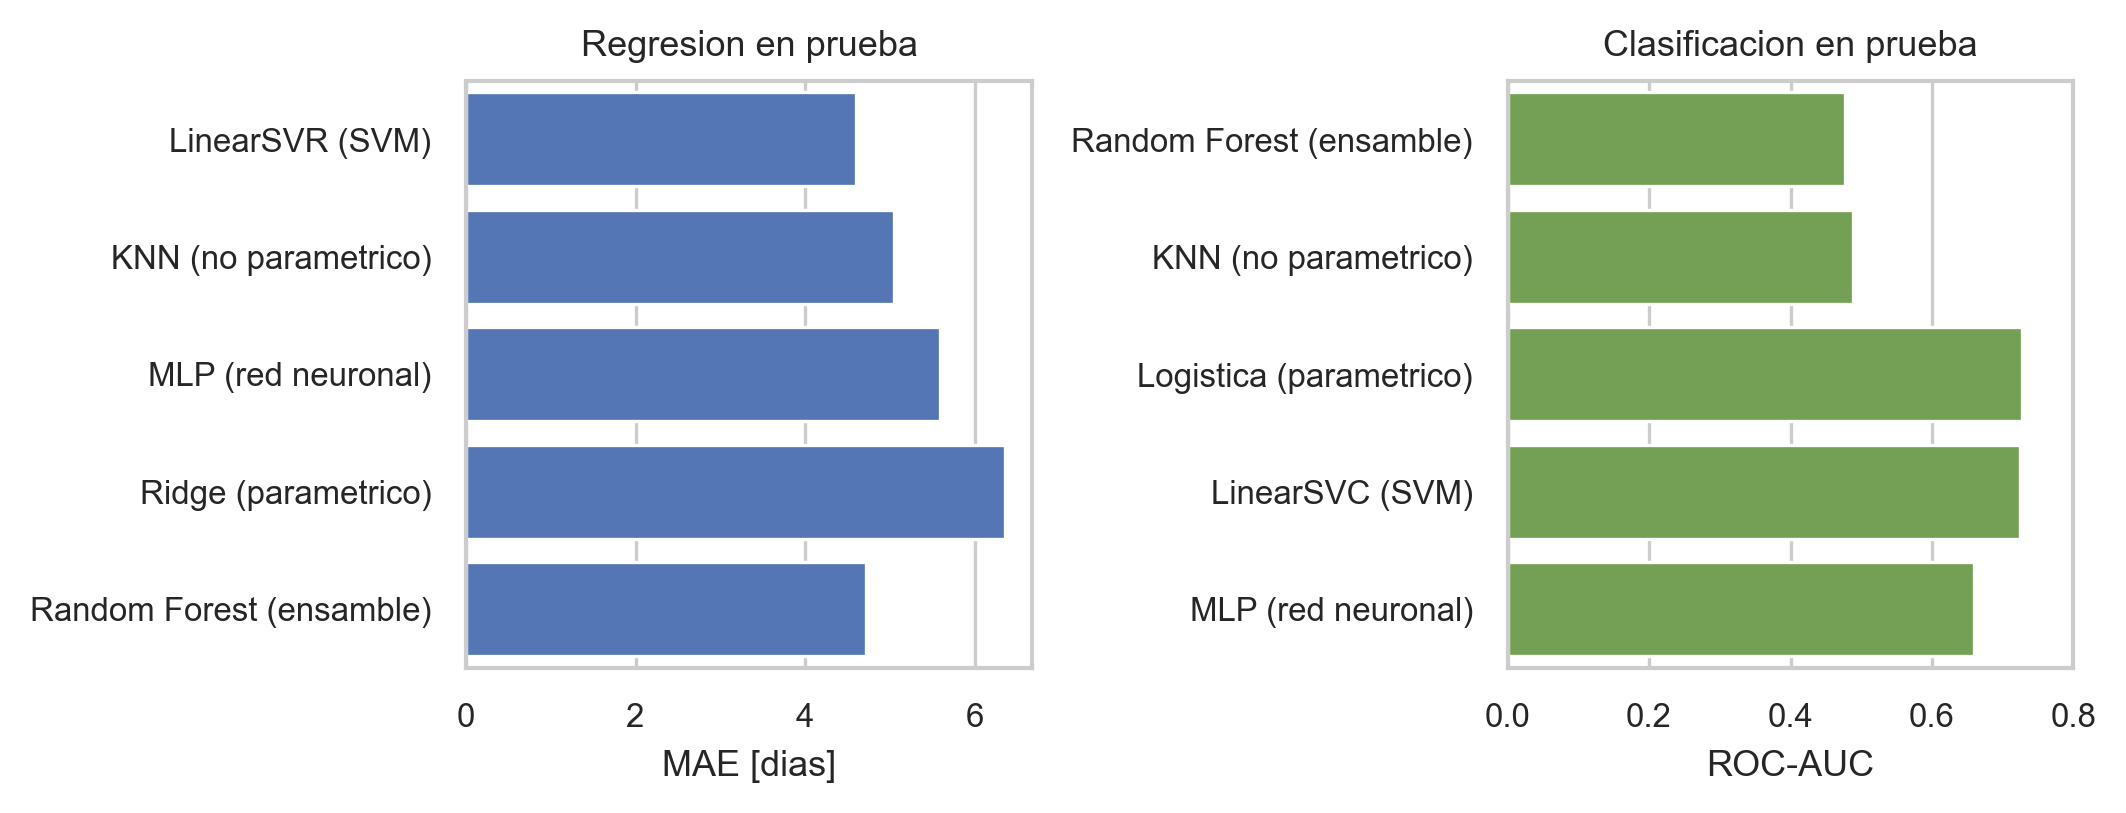
\includegraphics[width=\columnwidth]{model_results.png}
\caption{Resultados en prueba. Arriba: MAE de regresión (menor es mejor). Abajo: ROC--AUC de clasificación (mayor es mejor).}
\label{fig:models}
\end{figure}

\begin{table}[t]
\caption{Clasificación: ROC--AUC por partición y métricas de prueba.}
\label{tab:cls}
\centering\scriptsize
\begin{tabular}{lrrrrr}
\toprule
Modelo & AUC$_{tr}$ & AUC$_{val}$ & AUC$_{test}$ & BAcc & $F_1$ \\
\midrule
Random Forest & 0,980 & 0,686 & 0,477 & 0,505 & 0,080 \\
KNN & 1,000 & 0,620 & 0,488 & 0,500 & 0,000 \\
Logística & 0,748 & 0,605 & \textbf{0,727} & 0,603 & 0,130 \\
LinearSVC & 0,747 & 0,602 & 0,725 & \textbf{0,608} & \textbf{0,132} \\
MLP & 0,562 & 0,561 & 0,659 & 0,518 & 0,073 \\
\bottomrule
\end{tabular}
\end{table}

El bosque fue campeón de validación, pero cayó a ROC--AUC 0,477 (IC95\%: 0,434--0,518) en prueba, señal de deriva. Logística y SVC generalizaron mejor: detectaron 96,4\% de retrasos, aunque solo alrededor de 7\% de sus alertas fueron correctas. Por tanto, no debe usarse el umbral por defecto sin calibrarlo según el costo de falsas alarmas. La MLP tuvo la mayor precisión, pero omitió casi todos los retrasos.

\section{Reducción de dimensionalidad}
\subsection{Análisis individual}
La importancia por permutación del campeón de regresión fue dominada por \texttt{estimated\_delivery\_days} (0,698) y \texttt{customer\_state} (0,306); después aparecieron ciudad, mes, flete y categoría (0,022--0,033). En clasificación, la promesa estimada fue también la señal principal (0,089), seguida a distancia por día de semana, longitud del producto, cantidad y categoría (0,004--0,008). Variables con importancia cercana a cero son candidatas a eliminación, pero un valor negativo no prueba irrelevancia causal: puede surgir por colinealidad o deriva y debe confirmarse con ablación temporal.

\subsection{PCA y UMAP sobre los dos mejores modelos}
PCA retuvo 95\% de la varianza y redujo 80 variables transformadas a 27 (66,25\%). UMAP usó 10 componentes y redujo 87,5\%. Se aplicaron a LinearSVR y KNN en regresión, y a Random Forest y KNN en clasificación, seleccionados por validación. La Tabla~\ref{tab:red} compara prueba; UMAP se ajustó sin usar prueba y sus pequeñas variaciones entre ejecuciones son propias del método estocástico.

\begin{table}[t]
\caption{Reducción y desempeño de los dos mejores modelos por tarea.}
\label{tab:red}
\centering\scriptsize
\begin{tabular}{llrrr}
\toprule
Tarea & Método/modelo & Dim. & Red. & Métrica \\
\midrule
Reg. & PCA / LinearSVR & 27 & 66,3\% & MAE 4,86 \\
Reg. & PCA / KNN & 27 & 66,3\% & MAE 5,37 \\
Reg. & UMAP / LinearSVR & 10 & 87,5\% & MAE 4,67 \\
Reg. & UMAP / KNN & 10 & 87,5\% & MAE 5,74 \\
Clas. & PCA / RF & 27 & 66,3\% & AUC 0,573 \\
Clas. & PCA / KNN & 27 & 66,3\% & AUC 0,453 \\
Clas. & UMAP / RF & 10 & 87,5\% & AUC 0,517 \\
Clas. & UMAP / KNN & 10 & 87,5\% & AUC 0,524 \\
\bottomrule
\end{tabular}
\end{table}

\begin{figure}[t]
\centering
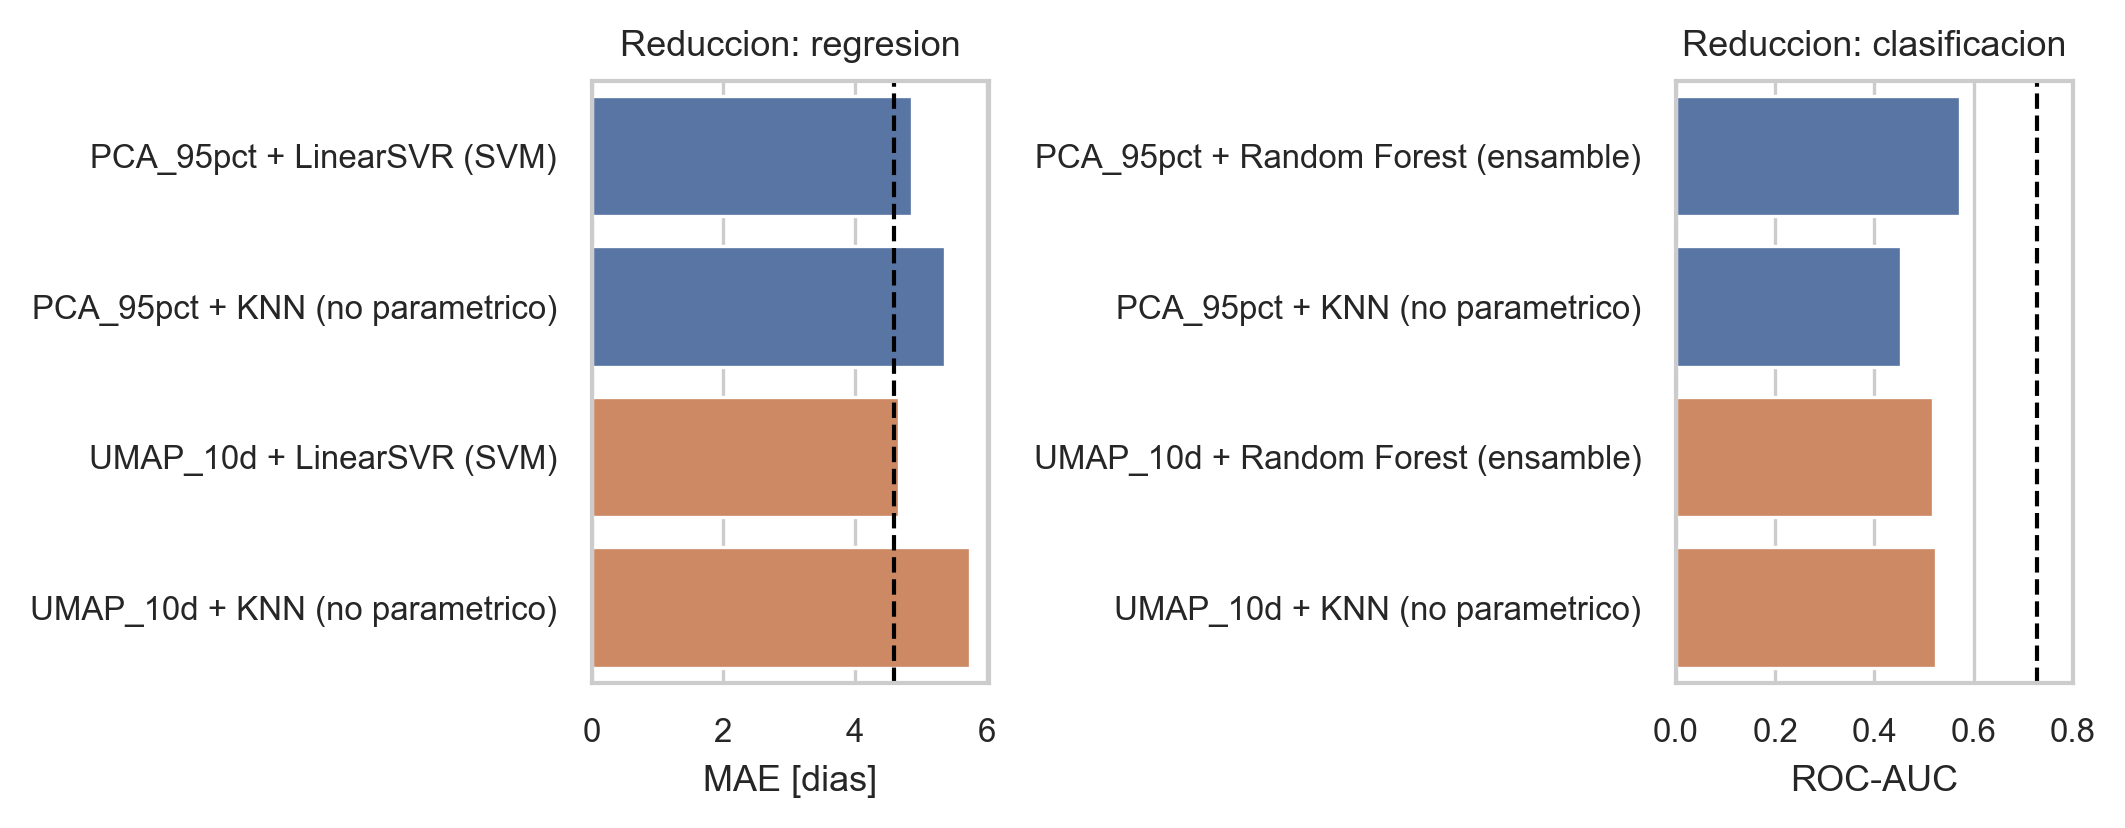
\includegraphics[width=\columnwidth]{reduction_results.png}
\caption{Desempeño después de PCA y UMAP. La línea punteada es el mejor modelo sin reducción.}
\label{fig:reduction}
\end{figure}

PCA aumentó 0,27 días el MAE de LinearSVR; UMAP retuvo mejor el desempeño con 70 variables menos, pero no superó de forma concluyente el IC del modelo completo. En clasificación ninguna reducción reparó la inestabilidad temporal. Se recomienda el espacio completo para máxima trazabilidad y UMAP solo cuando el costo computacional justifique sacrificar interpretabilidad.

\section{Reproducibilidad y solución completa}
El repositorio público contiene preprocesamiento, pruebas, tablas y figuras. El cuaderno ejecutable instala dependencias, descarga datos, entrena las diez configuraciones por tarea, calcula intervalos, ejecuta PCA/UMAP y exporta resultados. Puede abrirse directamente en
\begin{center}
\href{https://colab.research.google.com/github/Cde571/LogisTech-Modelos-Simulacion-II/blob/main/notebooks/03_entregable_ii_completo_colab.ipynb}{\textbf{Google Colab: Entregable II completo}}.
\end{center}
Código y trazabilidad: \url{https://github.com/Cde571/LogisTech-Modelos-Simulacion-II}. Para reproducir, se ejecutan todas las celdas en orden; las semillas están fijadas y cada tabla se genera desde los CSV de salida. El video de defensa de diez minutos debe presentar problema, método, resultados, reducción y conclusiones, y añadirse al repositorio cuando el equipo disponga del enlace.

\section{Conclusiones}
Se cumplieron las cinco familias de modelos, la separación entrenamiento--validación--prueba, intervalos de confianza, análisis individual y reducción con PCA y UMAP. LinearSVR fue la mejor opción para duración con error absoluto de 4,60 días. Para alertas, logística/SVC ofrecieron mejor discriminación futura que el bosque elegido en validación, pero la precisión baja exige calibración de umbral y monitoreo de deriva. UMAP comprimió 87,5\% conservando aproximadamente la regresión, mientras la reducción no benefició la clasificación. Antes de uso operativo se recomienda ampliar la búsqueda, recalibrar por ventana temporal y definir el costo empresarial de cada falsa alarma.

\bibliographystyle{IEEEtran}
\bibliography{references}
\end{document}
